\documentclass{article}
\usepackage[utf8]{inputenc}
\usepackage[english]{babel}
\usepackage{graphicx}
\usepackage{color}
\usepackage{amsfonts}

\def\warning#1{\color{red} #1 \color{black}}
\def\note#1{\color{cyan} #1 \color{black}}
\def\circled#1{\raisebox{.5pt}{\textcircled{\raisebox{-.9pt} {#1}}}}

\begin{document}

\title{Hoe los ik een examen Discrete Wiskunde op?}
\date{}
\author{}
\maketitle

\tableofcontents


Het examen Discrete Wiskunde verandert weinig en bestaat altijd uit zeven vragen. Zes van deze vragen zijn analoog met elke examenperiode en één vraag is willekeurig. In dit document wil ik technieken toelichten
om het examen sneller op te lossen. Dit gaat vooral over trukjes in Excel en de Antiview die je kan gebruiken in plaats van alles manueel te dien. 


\section{De Euclidische deling}
De Euclidische deling komt vaak voor dus is het verstanding om slechts een kleine stap te doen en excel de rest. Deze techniek werkt enkel bij een deling door twee gehele getallen. Veeltermen moet je nog altijd manueel delen. \warning{todo}

\section{Berekenen van een primitieve wortel}
Een primitieve wortel is het kleinste getal dat niet deelbaar is door een bepaald getal voor een bepaald veld. Het berekenen van een primitieve is heel eenvoudig. 
Er is slechts één gegeven nodig en dat is het veld. We nemen het volgende voorbeeld: Bereken de primitieve wortel over $\mathbb{Z}_{4051}.$

\begin{enumerate}
 \item Trek 1 af van het veldgetal en ontbindt dit in factoren. Gebruik het programma {\it factor} dat ook beschikbaar is op het examen. (Ingeven: {\sl factor 4050}) 
  $$4051 - 1 = 4050 = 2 * 3^{4} * 5^{2}$$
  Het getal 4050 wijst simpelweg op het aantal elementen in dit veld.
 \item We hebben het getal 4050 ontbonden in factoren. De bedoeling is om een excel-bestand op te maken zodat de primitieve wortel redelijk eenvoudig kan berekend worden. 
 Het excel-bestand heeft volgende opmaak:
 \begin{center}
  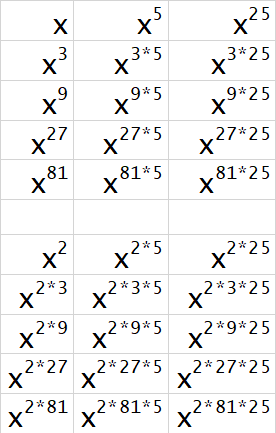
\includegraphics[height=5cm]{priem_wortel_1}
 \end{center}
 
 Dit stellen allemaal delers voor van het getal 4050. Nu is het de bedoeling dat we {\sl x} vervangen door oplopende getallen startend vanaf 2. \warning{todo}
 
 
 \subsection{De baby-step, giant-step techniek}
 De baby-step, giant-step techniek wordt gebruikt om een index van een getal ten opzichte van een primitieve wortel in een bepaald veld te berekenen. Hier moet de Euclidische deling ook uitgevoerd worden dus zorg dat je dit al goed kunt. Bij dit soort vraagstukken zijn er 3 gegevens. 
 \begin{itemize}
  \item {Het veld $\mathbb{Z}$} 
  \item {Een getal in dit veld waarvan de index moet berekend worden.}
  \item {De primitieve wortel $w$}
 \end{itemize}
 Op het examen zal er staan hoe groot één giant-step moet zijn. In dit voorbeeld nemen we giant-steps die 10 baby-steps groot zijn. We beschouwen het veld $\mathbb{Z}_{71}$ en de primitieve wortel $w = 7$. We willen de index van 5 berekenen. Begin met de eerste 10 baby-steps te genereren. Je begint met de primitieve wortel, en daarna gebruik je Formule 1. De letter b stelt de n-de baby-step voor. Bekijk ook Figuur \ref{fig:babystep_giantstep_1} waarop dit gevisualiseerd staat(p. \pageref{fig:babystep_giantstep_1}).
 $$b_n = b_{n-1} * w\; \% \;71 \eqno(1)$$
 
\begin{figure}
  \begin{center}
  \caption{Voorstelling van Formule 1 voor de berekening van de baby-steps}
  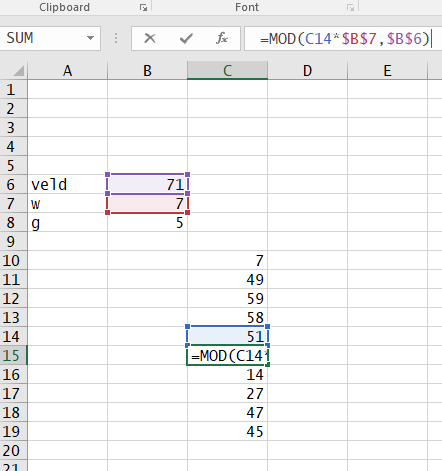
\includegraphics[width=\textwidth]{babystep_giantstep_1}
  \label{fig:babystep_giantstep_1}
  \end{center}
  
\end{figure}
  
 
Nadat de eerste 10 baby-steps genereerd zijn moet je het inverse element, ten opzichte van 71, van de laatste baby-step bepalen. Dit doe je door het algoritme van Euclides toe te passen(Figuur \ref{fig:babystep_giantstep_2}).

\begin{figure}
  \begin{center}
  \caption{Algoritme van Euclides bij de baby-step, giant-step techniek}
  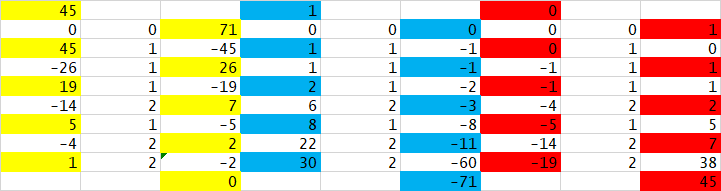
\includegraphics[width=\textwidth]{babystep_giantstep_2}
  \label{fig:babystep_giantstep_2}
  \end{center}
\end{figure}
Het inverse element is hier dus 30. Nu moeten de giant-steps gegenereerd worden. Je vertrekt vanaf het getal waarvan we de index zoeken. Daarna gebruik je Formule 1 maar vervang je de baby-step door de giant-step. Dit wordt voorgesteld in Figuur \ref{fig:babystep_giantstep_3}.


\begin{figure}
  \begin{center}
  \caption{Voorstelling van Formule 1 voor de berekening van de giant-steps}
  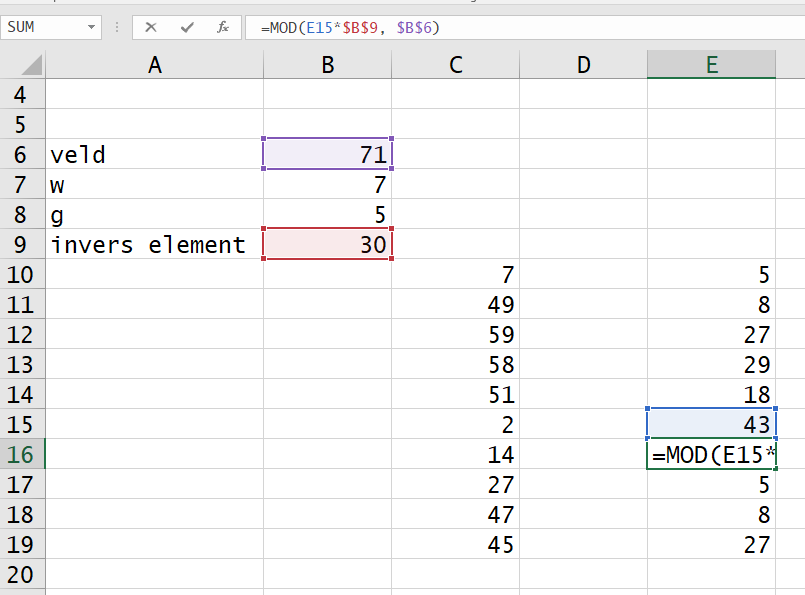
\includegraphics[width=\textwidth]{babystep_giantstep_3}
  \label{fig:babystep_giantstep_3}
  \end{center}
\end{figure}
  
Merk op dat het getal 27 zowel bij de baby-steps als bij de giant-steps voorkomt. Dit stelt de index voor die we zoeken. Het getal 27 is het achtste getal in de baby-step verzameling. Bij de giant-step verzameling is dit het derde getal. Aangezien elke giant-step een grootte heeft van tien babysteps, wordt dit nog eens vermenigvuldigd met tien. De index wordt $$8 + (3 * 10) = 8 + 30 = 38$$
De oplossing is formeel: De index van 5 over het veld $\mathbb{Z}_{71}$ met primitieve wortel $w = 7$ is 38. Er zijn 3 giant-steps nodig en 8 baby-steps.

\subsection{Elliptische krommen}
 
\end{enumerate}




\end{document}
